\chapter{Dynamic Model of the Quadrotor \label{ch:model}}
tgrtnrttrr
\section{Quadrotors' Configurations}
\url{https://www.google.com/search?q=why+\%2B+or+x+configuration+quadcopter&ie=utf-8&oe=utf-8&client=firefox-b-ab&gfe_rd=cr&dcr=0&ei=Mr0BWrW9HtHk8AfXm7fADQ}
\\\\
\url{https://community.micro-motor-warehouse.com/t/vs-x-configuration/2673}
\\\\
\url{https://www.quora.com/Why-is-x-configuration-preferred-over-+-config-of-quadcopter}
\\\\
\url{https://www.rcgroups.com/forums/showthread.php?1203569-Quad-X-vs-configuration}


\subsection{'+' Configuration}
rtgrtgtrbrtgrg
\begin{figure*}
\begin{center}
% Use the relevant command to insert your figure file.
% For example, with the graphicx package use
  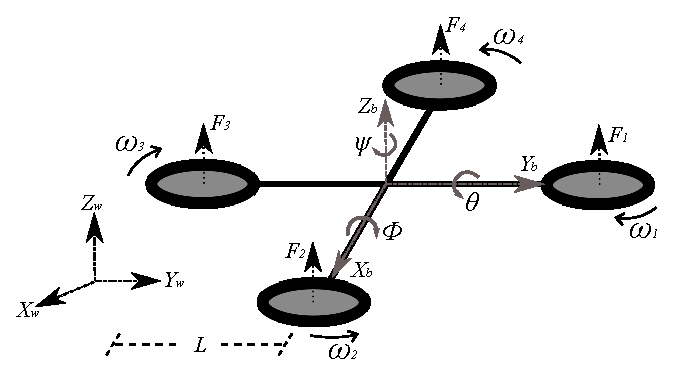
\includegraphics[width=0.83\textwidth]{quadcopterplus.eps}
% figure caption is below the figure
\caption{Quadrotor squeme with movement axis and thrust forces.} 
    \label{fig:quadcopterplus}
    \end{center}
\end{figure*}
\subsection{'X' Configuration}
sdsfsdfsfs
\begin{figure*}
\begin{center}
% Use the relevant command to insert your figure file.
% For example, with the graphicx package use
  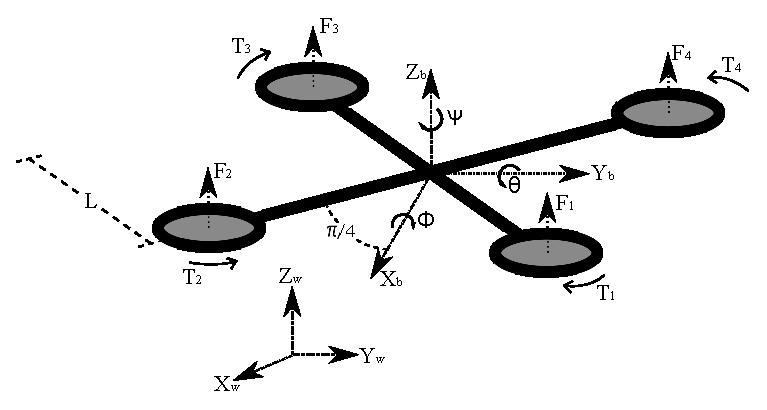
\includegraphics[width=0.9\textwidth]{quadcopter1.eps}
% figure caption is below the figure
\caption{Quadrotor squeme with movement axis and thrust forces.} 
    \label{fig:marcoreferencia}
    \end{center}
\end{figure*}

\section{Nonlinear Model}

This section describes the dynamic modeling used to perform the quadrotor control, based on the study carried out in \cite{modelamiento, modelamientoPDAFC, modelamientoNCQ}. This model represents the quadrotor as a solid symmetrical object subject to a total thrust and three torques, without considering the dynamics of the actuators.


\subsection{Euler-Lagrange Approach}
The general coordinates representing the position and attitude of the quadrotor are defined as
\begin{equation}
	q=\begin{bmatrix}
	\xi & \eta
	\end{bmatrix}^{T},
	\label{ec:coorgenerales}
\end{equation}
where $\xi=\begin{bmatrix}
x & y & z
\end{bmatrix}^{T}$ is the vector representing the position of the center of mass of the quadrotor relative to the body reference frame shown in Fig. \ref{fig:marcoreferencia} and $\eta=\begin{bmatrix}
\psi & \theta & \phi
\end{bmatrix}^{T}$ represent the quadrotor's attitude.
\\\\
The Lagrangian of the quadrotor is defined by
\begin{equation}
	L(q,\dot{q})=K_{trans}+K_{rot} - U,	
	\label{ec:lagrangiano}
\end{equation}
where $ K_{trans} = \dfrac{m}{2}\dot{\xi}^{T}\dot{\xi} $ is the translational kinetic energy, $ K_{rot} = \dfrac{1}{2}\dot{\eta}^{T}J\dot{\eta} $ is the rotational kinetic energy, $ U=mgz $ is the potential energy, $m$ is the quadrotor's mass , $z$ is the quadrotor's elevation, $g$ is the gravity acceleration magnitude, and $J$ is the inertial matrix. The dynamic model of the quadrotor is derived from the Euler-Lagrange equation
\begin{equation}
	\dfrac{d}{dt}\dfrac{\partial L}{\partial \dot{q}}-\dfrac{\partial L}{\partial q}=
	\begin{bmatrix}
	F_{\xi}\\
	\tau
	\end{bmatrix},
	\label{ec:eulerlag}
 \end{equation} 
where $F_{\xi}=R_{b}^{w}\hat{F_{b}}$ is the translational force applied to the quadrotor by the four motors, $\tau$ contains the rolling, pitching and yawing torques, and 
\begin{equation}
R_{b}^{w} = \begin{bmatrix}
c\theta c\psi & c\psi s\theta s\phi-c\phi s\psi & s\phi s\psi+c\phi c\psi s\theta\\
c\theta s\psi & s\psi s\theta s\phi+c\phi c\psi & c\phi s\psi s\theta - s\phi c\psi\\
-s\theta & c\theta s\phi & c\theta c\phi
\end{bmatrix}
\end{equation}
is the rotation matrix from the body to the Earth frame where $c\theta = \cos\theta$ and $s\theta = \sin\theta$.
\\\\
In the quadrotor's body frame, the translational force $\hat{F_{b}}$ is only applied in the $z_{b}$ axis as shown in Fig. \ref{fig:marcoreferencia}. This force is represented by
\begin{equation}
	\hat{F_{b}}=\begin{pmatrix}
	0\\
	0\\
	u
	\end{pmatrix} = \begin{pmatrix}
	0\\
	0\\
	\sum_{i=1}^{4}F_{M_i}
	\end{pmatrix}  ,
 \label{ec:fuerzas}
 \end{equation} 
with $ F_{M_i} $ being the force, in N, exerted by the motor $ M_{i}$, as shown in Fig. \ref{fig:marcoreferencia}.
\\\\
The force $ F_{M_i} $ has a linear dependency with the square of the motor angular velocity, defined as
\begin{equation}
	F_{M_i}=k_{i}w_{i}^{2},
	\label{ec:fi}
\end{equation}
where $ w_{i} $ is the angular velocity of the motor, and $ k_{i} $ is a proportional constant. However, in practice $F_{M_i}$ must be set using the PWM signal input of an ESC. The thrust-PWM relation is found experimentally and is shown in Section \ref{sec:Implementation}.
\\\\
The Euler-Lagrange equations can be divided in two parts, one for the $\xi$ coordinates and another for the $\eta$ coordinates, getting
\begin{equation}
\label{eqn:E-L1}
\ddot{\xi} =
\begin{bmatrix}
\ddot{x} \\ \ddot{y} \\ \ddot{z}
\end{bmatrix} 
=
\begin{bmatrix}
\frac{u_{1}}{m}(\cos\phi\sin\theta\cos\psi + \sin\phi\sin\psi) \\
 \frac{u_{1}}{m}(\cos\phi\sin\theta\sin\psi - \sin\phi\cos\psi) \\
\frac{u_{1}}{m}(\cos\phi\cos\theta) - g
\end{bmatrix},
\end{equation}
\begin{equation}
\label{eqn:E-L2}
\ddot{\eta} =
\begin{bmatrix}
\ddot{\psi} \\ \ddot{\theta} \\ \ddot{\phi}
\end{bmatrix} 
 =
\begin{bmatrix}
\dot{\phi}\dot{\theta}\dfrac{J_{xx}-J_{yy}}{J_{zz}} + \dfrac{u_{2}}{J_{zz}} \\
\dot{\phi}\dot{\psi}\dfrac{J_{zz}-J_{xx}}{J_{yy}} + \dfrac{u_{3}}{J_{yy}} \\
 \dot{\theta}\dot{\psi}\dfrac{J_{yy}-J_{zz}}{J_{xx}} +  \dfrac{u_{4}}{J_{xx}}
\end{bmatrix},
\end{equation}
where, $\begin{bmatrix}
u_{1},\ u_{2},\ u_{3}, \ u_{4}
\end{bmatrix}^{T} = \begin{bmatrix}
u,\ \tau_{\psi},\ \tau_{\theta},\ \tau_{\phi}
\end{bmatrix}^{T} $, and $ (J_{xx}, J_{yy}, J_{zz}) $ are the moments of inertia around the quadrotor's body axes \cite{Emam2016, Badr2016}.
\\\\

that is a simplified representation of the quadrotor complete model found in \cite{Bouabdallah2007}.

\subsection{Newton-Euler Approach}
sdasdasdaasd

\section{Linearized Model}
\setcounter{MaxMatrixCols}{20}
\cite{Sabatino2015}
\\\\
The Euler-Lagrange equations in (\ref{eqn:E-L1}) and (\ref{eqn:E-L2}) are linearized using their Jacobian around the hover state where $\begin{bmatrix}
\eta,\ \dot{\eta},\ \dot{\xi}
\end{bmatrix} \to \begin{bmatrix}
0,\ 0,\ 0
\end{bmatrix}$, getting
\begin{equation}
\label{eqn:linear}
\ddot{q}
=
\begin{bmatrix}
g\theta \\
g\phi\\
u_{1}/m \\
u_{2}/J_{zz} \\
u_{3}/J_{yy} \\
u_{4}/J_{xx}
\end{bmatrix},
\end{equation}

As said above, in order to perform the linearization, an equilibrium point is
needed. Such an equilibrium point can be:
\begin{equation}
\overline{\mathbf{x}} = \begin{bmatrix}
\overline{x} & \overline{y} & \overline{z} & 0 & 0 & 0 & 0 & 0 & 0 & 0 & 0 & 0
\end{bmatrix}^{T}
\end{equation}
From the equations, we can find that the equilibrium point (2.29) is obtained by
the constant input value:
\begin{equation}
\overline{\mathbf{u}} = \begin{bmatrix}
mg & 0 & 0 & 0
\end{bmatrix}^{T}
\end{equation}
with $mg$ being the lift force.
\\\\
The linearized model of the quad-rotor helicopter written as a state space model is given by

\begin{align*}
\dot{\mathbf{x}}(t) = & A\mathbf{x}(t)+B\mathbf{u}(t),\\
\mathbf{y}(t) = & C\mathbf{x}(t),
\end{align*}
where
\begin{align}
\begin{split}
A  = \frac{\partial f(\mathbf{x},\mathbf{u})}{\partial \mathbf{x}}\Bigr|_{\substack{\mathbf{x}=\overline{\mathbf{x}}\\\mathbf{u}=\overline{\mathbf{u}}}} = & 
\begin{bmatrix}
0 & 1 & 0 & 0 & 0 & 0 & 0 & 0 & 0 & 0 & 0 & 0\\[2px]
0 & 0 & 0 & 0 & 0 & 0 & 0 & 0 & g & 0 & 0 & 0\\[2px]
0 & 0 & 0 & 1 & 0 & 0 & 0 & 0 & 0 & 0 & 0 & 0\\[2px]
0 & 0 & 0 & 0 & 0 & 0 & 0 & 0 & 0 & 0 & g & 0\\[2px]
0 & 0 & 0 & 0 & 0 & 1 & 0 & 0 & 0 & 0 & 0 & 0\\[2px]
0 & 0 & 0 & 0 & 0 & 0 & 0 & 0 & 0 & 0 & 0 & 0\\[2px]
0 & 0 & 0 & 0 & 0 & 0 & 0 & 1 & 0 & 0 & 0 & 0\\[2px]
0 & 0 & 0 & 0 & 0 & 0 & 0 & 0 & 0 & 0 & 0 & 0\\[2px]
0 & 0 & 0 & 0 & 0 & 0 & 0 & 0 & 0 & 1 & 0 & 0\\[2px]
0 & 0 & 0 & 0 & 0 & 0 & 0 & 0 & 0 & 0 & 0 & 0\\[2px]
0 & 0 & 0 & 0 & 0 & 0 & 0 & 0 & 0 & 0 & 0 & 1\\[2px]
0 & 0 & 0 & 0 & 0 & 0 & 0 & 0 & 0 & 0 & 0 & 0
\end{bmatrix} \\[15px]
B = \frac{\partial f(\mathbf{x},\mathbf{u})}{\partial \mathbf{u}}\Bigr|_{\substack{\mathbf{x}=\overline{\mathbf{x}}\\\mathbf{u}=\overline{\mathbf{u}}}} = & 
\begin{bmatrix}
0 & 0 & 0 & 0 & 0 & \frac{1}{m} & 0 & 0 & 0 & 0 & 0 & 0\\[5px]
0 & 0 & 0 & 0 & 0 & 0 & 0 & \frac{1}{I_{zz}} & 0 & 0 & 0 & 0\\[5px]
0 & 0 & 0 & 0 & 0 & 0 & 0 & 0 & 0 & \frac{1}{I_{yy}} & 0 & 0\\[5px]
0 & 0 & 0 & 0 & 0 & 0 & 0 & 0 & 0 & 0 & 0 & \frac{1}{I_{xx}}
\end{bmatrix}^T \\[15px]
C = &
\begin{bmatrix}
1 & 0 & 0 & 0 & 0 & 0 & 0 & 0 & 0 & 0 & 0 & 0\\
0 & 0 & 1 & 0 & 0 & 0 & 0 & 0 & 0 & 0 & 0 & 0\\
0 & 0 & 0 & 0 & 1 & 0 & 0 & 0 & 0 & 0 & 0 & 0\\
0 & 0 & 0 & 0 & 0 & 0 & 1 & 0 & 0 & 0 & 0 & 0 
\end{bmatrix}
\end{split}
\end{align}

with the parameters  

$m=0.64 $ kg, 

$g=9.81$ m/s.


The state vector is defined as

\begin{align*}
x(t)=&
\begin{bmatrix}
r_x & \dot{r}_x & r_y & \dot{r}_y & r &\dot{r}_z 
\end{bmatrix}^T,
\end{align*}
and the control inputs as
\begin{align*}
u(t)=&
\begin{bmatrix}
u_1 & u_2 &u_3 & u_4
\end{bmatrix}^T,
\end{align*}

and the output vector is defined as

\begin{align*}
r(t)=
\begin{bmatrix}
r_{x} & r_{y} & r_{z}
\end{bmatrix}^T.
\end{align*}

\section{Quadrotor's Inputs Setting}
\label{sec:inputsetting}


\subsection{Inputs in '+' Configuration}
\begin{equation}
	\tau = \begin{bmatrix}
	\tau_{\psi}\\[5pt]
	\tau_{\theta}\\[5pt]
	\tau_{\phi}
	\end{bmatrix} = \begin{bmatrix}
								T_{2} + T_{4} - T_{1} - T_{3}\\[5pt]
								L(F_{4}-F_{2})\\[5pt]
								L(F_{3}-F_{1})
							\end{bmatrix},
	\label{ec:torques2}						
\end{equation}
\subsection{Inputs in 'X' Configuration}
The rolling, pitching and yawing torques contained in vector $\tau$, are generated using the force exerted by each motor as 
\begin{equation}
	\tau = \begin{bmatrix}
	\tau_{\psi}\\[5pt]
	\tau_{\theta}\\[5pt]
	\tau_{\phi}
	\end{bmatrix} = \begin{bmatrix}
								T_{2} + T_{4} - T_{1} - T_{3}\\[5pt]
								L \cos\left(\dfrac{\pi}{4}\right)(F_{3}+F_{4}-F_{2}-F_{1})\\[10pt]
								L \cos\left(\dfrac{\pi}{4}\right)(F_{2}+F_{3}-F_{1}-F_{4})
							\end{bmatrix},
	\label{ec:torques}						
\end{equation}
where $ T_{i} $ is the torque produced by each motor along the $z_{b}$ axis, $ L $ is the distance between each motor's rotor and the quadrotor's center of mass, and $L cos(\pi/4)$ is the real distance between the point of application of the rolling and pitching torques and the quadrotor's center of mass along the $x_b$ and $y_b$ axes \cite{Faessler2016}.\\\\

\subsection{Thrust Compensation}
\url{https://robotics.stackexchange.com/questions/4247/tilt-compensated-motor-output-to-keep-altitude-for-quadcopter}
Recalling the rotation matrix $R_{b}^{w}$,
\begin{equation}
R_{b}^{w} = \begin{bmatrix}
c\theta c\psi & c\psi s\theta s\phi-c\phi s\psi & s\phi s\psi+c\phi c\psi s\theta\\
c\theta s\psi & s\psi s\theta s\phi+c\phi c\psi & c\phi s\psi s\theta - s\phi c\psi\\
-s\theta & c\theta s\phi & c\theta c\phi
\end{bmatrix}
\end{equation}
\begin{equation}
u = u^{*} \cos{\theta}\cos{\phi}
\end{equation}
\begin{equation}
u^{*} = \dfrac{u}{\cos{\theta}\cos{\phi}}
\end{equation}
\section{Conclusions}
This chapter presented the design of the two vehicles developed in this thesis.
The test-bench and the OS4. The first system is only capable of 3 DoF which
facilitates the testing of the controllers. However, it is possible to detach the
flying part in order to test free flights. Before designing the second system
which is a free flying quadrotor, a new design methodology is introduced. It
allows an optimal design of small-scale rotorcraft. Four new design indicators
were introduced for a precise and complete evaluation of the design performance.
This methodology appreciably facilitated the components selection
process and battery dimensioning of OS4. This quadrotor exhibits higher
capabilities and endurance than the competition. This is verified through
the comparison of different design parameters. OS4 embeds all the necessary
avionics and energy devices for a fully autonomous flight. This comprises a
low cost IMU, a vision based position sensor specifically developed for this
project and an obstacle detection setup.

